%\documentclass{beamer}

\documentclass[handout]{beamer}
 
\usepackage[utf8]{inputenc}
\usepackage{graphicx}
\usepackage{wrapfig}
\usepackage{lipsum}
\usepackage{hyperref}
\usepackage{tabularx}
\usepackage{amsmath}
\usepackage{enumerate}
\usepackage[utf8]{inputenc}
\usepackage{tikz}
\usepackage{circuitikz}
\usepackage{xcolor}

\usepackage{pgfpages}

%\mode<handout>{%
%    \pgfpagesuselayout{4 on 1}[letter] 
%    \setbeameroption{show notes}
%}

\renewcommand{\vec}[1]{\mathbf{#1}} % Display vectors as boldface %

\let\oldhat\hat   % Also display hats as boldface
\renewcommand{\hat}[1]{\oldhat{\mathbf{#1}}} % Also display hats as boldface
 
%Information to be included in the title page:
\title{Physics 231}
\subtitle{Lecture 3: Op Amps I}
\author{Eric Landahl}
\institute{DePaul University Physics Department}
 
\begin{document}
 
\frame{\titlepage}

\begin{frame}
\frametitle{Table of Contents}
\tableofcontents
\end{frame}}
%%%%%%%%%%%%%%%%%%%%
\section{Thevenin Equivalent Circuits}
%%%%%%%%%%%%%%%%%%%%
\subsection{Analysis}
%%%%%%%%%%%%%%%%%%%%
\begin{frame}{\secname : \subsecname}
    Replace the entire source with a "black box" with an equivalent voltage and an equivalent resistance in series.
    \begin{figure}
    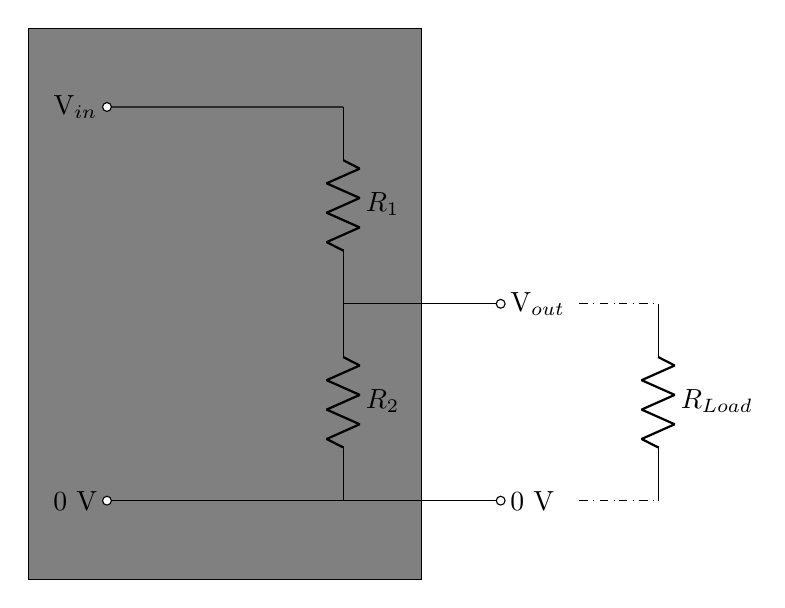
\begin{tikzpicture}
        % Gray backgorund box (can be commented out)
        \draw [fill=gray] (0,4.5) rectangle (5,11.5);
        % Voltage divider
        \draw (4,10.5) to[short,-o] (1,10.5); % Connect to 5 V DC
        \draw (1,10.5) node[anchor=east] {V$_{in}$};
        \draw  (4,10.5) to[R=$R_1$] (4,8);
        \draw (6,8) node[anchor=west] {V$_{out}$};
        \draw (4,8) to[short,-o] (6,8);
        \draw (4,8) to[R=$R_2$] (4,5.5);
        \draw (4,5.5) to[short,-o] (1,5.5); 
        \draw (1,5.5) node[anchor=east] {0 V};
        \draw (4,5.5) to[short,-o] (6,5.5);
        \draw (6,5.5) node[anchor=west] {0 V};
        % Load resistor (can be commented out)
        \draw [dash dot] (7,5.5) to[short](8,5.5);
        \draw [dash dot] (7,8) to[short](8,8);
        \draw (8,8) to[R=$R_{Load}$] (8,5.5);
    \end{tikzpicture}
    \end{figure}
\end{frame}
%%%%%%%%%%%%%%%%%%%%
\begin{frame}{\secname : \subsecname}
    The ``Thevenin Equivalent'' Circuit is defined to be the one where the output voltage $V_{out}=\frac{V_{th}}{2}$  when connected to a load $R_{Load}=R_{th}$.  \emph{Every power supply has a $V_{th}$ and $R_{th}$.}
    \begin{figure}
    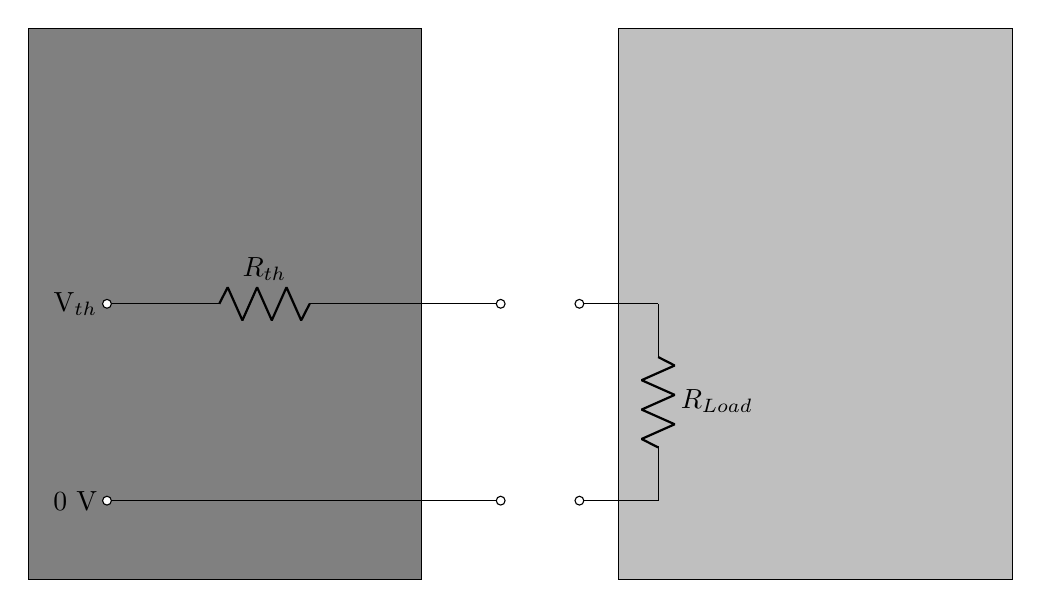
\begin{tikzpicture}
        % Source
        % Gray backgorund box (can be commented out)
        \draw [fill=gray] (0,4.5) rectangle (5,11.5);
        \draw (2,8) to [short,-o] (1,8);
        \draw (2,8) to[R=$R_{th}$] (4,8); % Connect to 5 V DC
        \draw (1,8) node[anchor=east] {V$_{th}$};
        \draw (4,8) to[short,-o] (6,8);
        \draw (4,5.5) to[short,-o] (1,5.5); 
        \draw (1,5.5) node[anchor=east] {0 V};
        \draw (4,5.5) to[short,-o] (6,5.5);
        % Load 
        \draw [fill=lightgray] (7.5,4.5) rectangle (12.5,11.5);
        \draw (8,5.5) to[short,-o](7,5.5);
        \draw (8,8) to[short,-o](7,8);
        \draw (8,8) to[R=$R_{Load}$] (8,5.5);
    \end{tikzpicture}
    \end{figure}
\end{frame}
%%%%%%%%%%%%%%%%%%%%
\begin{frame}{\secname : \subsecname}
    Step 1: Determine the voltage across the outputs without the load attached (as an open circuit).  This open circuit voltage is $V_{th}$. \emph{Remember, the voltmeter draws no current.}
    \begin{figure}
    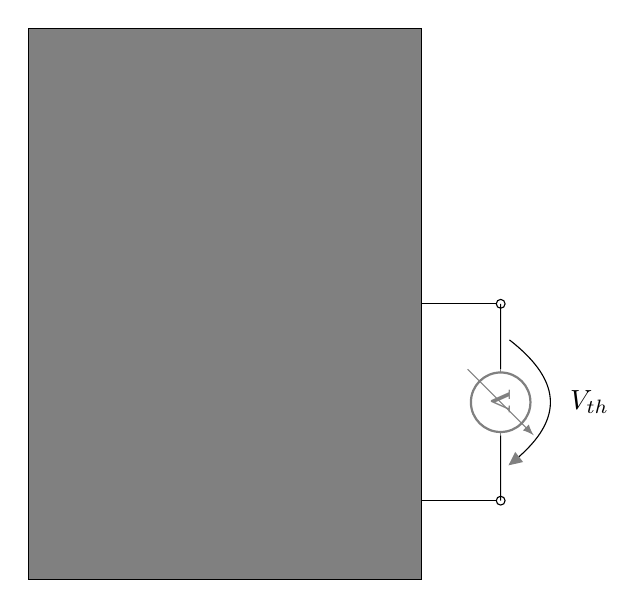
\begin{tikzpicture}
        % Source
        % Gray backgorund box (can be commented out)
        \draw [fill=gray] (0,4.5) rectangle (5,11.5);
        \draw (5,8) to[short,-o] (6,8);
        \draw (5,5.5) to[short,-o] (6,5.5);
        % Voltmeter
        \draw (6,8) to[voltmeter,color=gray,v^>=$V_{th}$] (6,5.5); % Show ammeter 
    \end{tikzpicture}
    \end{figure}
\end{frame}
%%%%%%%%%%%%%%%%%%%%
\begin{frame}{\secname : \subsecname}
    Step 2: Determine the current through the outputs when they are shorted.  This short circuit current is $I_{sc}$. \emph{Remember, the ammeter has zero resistance and is a short.}
    \begin{figure}
    \begin{tikzpicture}
        % Source
        % Gray backgorund box (can be commented out)
        \draw [fill=gray] (0,4.5) rectangle (5,11.5);
        \draw (5,8) to[short,-o] (6,8);
        \draw (5,5.5) to[short,-o] (6,5.5);
        % Voltmeter
        \draw (6,8) to[ammeter,color=gray,i=^$I_{sc}$] (6,5.5); % Show ammeter 
    \end{tikzpicture}
    \end{figure}
\end{frame}
%%%%%%%%%%%%%%%%%%%%
\begin{frame}{\secname : \subsecname}
    Step 3.  Calculate the equivalent (or source, or Thevenin) resistance by dividing the open-circuit voltage by the short-circuit current.
    \begin{equation}
        R_{th}=\dfrac{V_{th}}{I_{sc}}
    \end{equation}
    \begin{figure}
    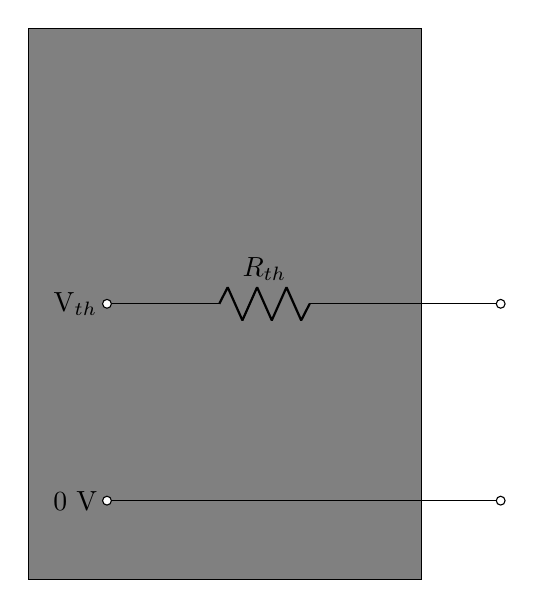
\begin{tikzpicture}
        % Source
        % Gray backgorund box (can be commented out)
        \draw [fill=gray] (0,4.5) rectangle (5,11.5);
        \draw (2,8) to [short,-o] (1,8);
        \draw (2,8) to[R=$R_{th}$] (4,8); % Connect to 5 V DC
        \draw (1,8) node[anchor=east] {V$_{th}$};
        \draw (4,8) to[short,-o] (6,8);
        \draw (4,5.5) to[short,-o] (1,5.5); 
        \draw (1,5.5) node[anchor=east] {0 V};
        \draw (4,5.5) to[short,-o] (6,5.5);
    \end{tikzpicture}
    \end{figure}
\end{frame}
%%%%%%%%%%%%%%%%%%%%
\begin{frame}{\secname : \subsecname}
    Step 4.  The output voltage $V_{out}$ can now be determined for any load resistance $R_{Load}$ by using the voltage divider equation.
    \begin{equation}
        V_{out}=\left( \dfrac{R_{Load}}{R_{Load}+R_{th}} \right) V_{th}
    \end{equation}
    \begin{figure}
    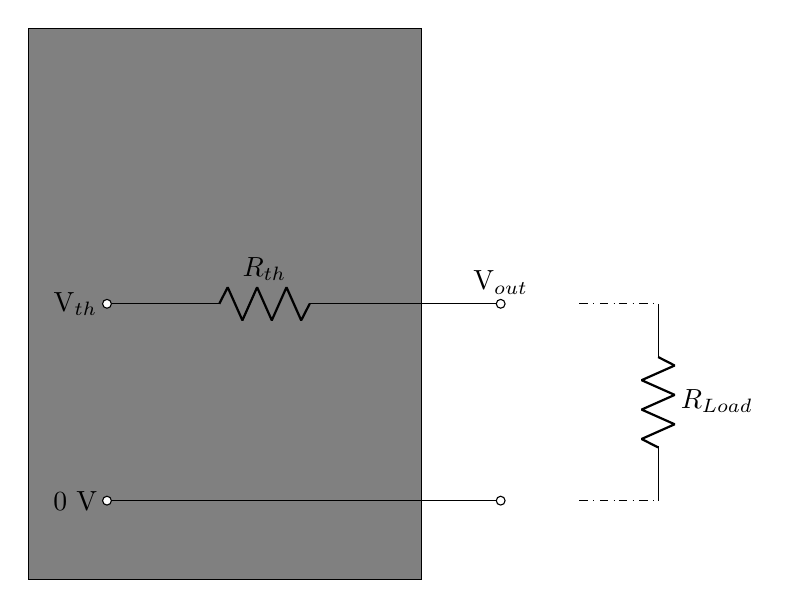
\begin{tikzpicture}
        % Source
        % Gray backgorund box (can be commented out)
        \draw [fill=gray] (0,4.5) rectangle (5,11.5);
        \draw (2,8) to [short,-o] (1,8);
        \draw (2,8) to[R=$R_{th}$] (4,8); % Connect to 5 V DC
        \draw (1,8) node[anchor=east] {V$_{th}$};
        \draw (4,8) to[short,-o] (6,8);
        \draw (4,5.5) to[short,-o] (1,5.5); 
        \draw (1,5.5) node[anchor=east] {0 V};
        \draw (4,5.5) to[short,-o] (6,5.5);
        % Load resistor
        \draw (6,8) node[anchor=south] {V$_{out}$};
        \draw [dash dot] (7,5.5) to[short](8,5.5);
        \draw [dash dot] (7,8) to[short](8,8);
        \draw (8,8) to[R=$R_{Load}$] (8,5.5);
    \end{tikzpicture}
    \end{figure}
\end{frame}
%%%%%%%%%%%%%%%%%%%%
\begin{frame}{\secname : \subsecname}
    Special cases of load resistance:
    \begin{equation}
        V_{out}=\left( \dfrac{R_{Load}}{R_{Load}+R_{th}} \right) V_{th}
    \end{equation}
    \begin{enumerate}
        \item If $R_{Load} = \infty$ (no load), the circuit is open and $V_{out}=V_{th}$
        \item If $R_{Load} = 0$, the circuit is shorted and $V_{out}=0$
        \item If $R_{Load} = R_{th}$ then $V_{out}=\dfrac{V_{th}}{2}$
        \item If $R_{Load} \gg R_{th}$ then $V_{out}=V_{th}$, or a ``good load''
        \item If $R_{Load} \approx R_{th}$ then $V_{out}<V_{th}$, or a ``poor load''
    \end{enumerate}
    \vspace{0.5 cm}
    Always check your answer by Property 3:  \\
    Loading with the source resistance halves the output voltage.
\end{frame}
%%%%%%%%%%%%%%%%%%%%
\subsection{The Voltage Divider Source}
%%%%%%%%%%%%%%%%%%%%
\begin{frame}{\secname : \subsecname}
    \begin{equation}
        \dfrac{1}{R_{th}}=\dfrac{1}{R_{1}}+\dfrac{1}{R_{2}}
        \qquad or \qquad
        R_{th}=\dfrac{R_1 R_2}{R_1+R_2}
    \end{equation}
    \begin{figure}
    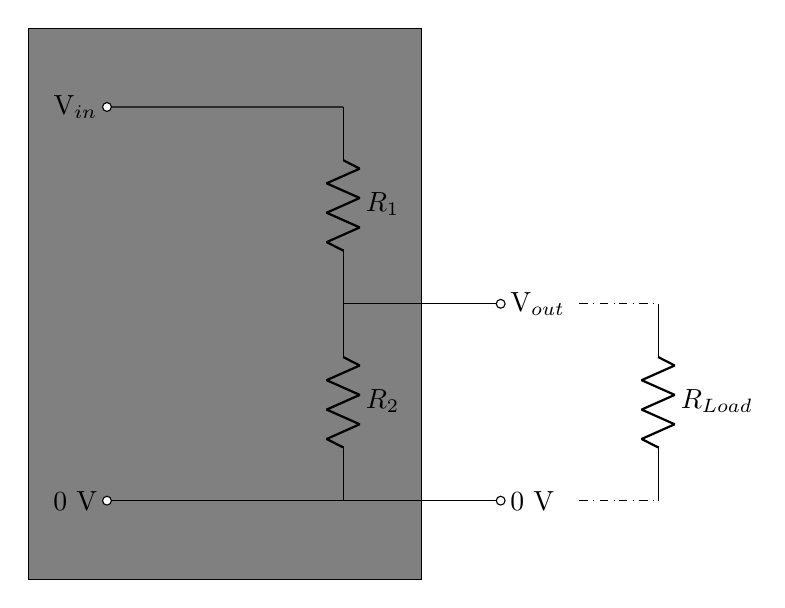
\begin{tikzpicture}
        % Gray backgorund box (can be commented out)
        \draw [fill=gray] (0,4.5) rectangle (5,11.5);
        % Voltage divider
        \draw (4,10.5) to[short,-o] (1,10.5); % Connect to 5 V DC
        \draw (1,10.5) node[anchor=east] {V$_{in}$};
        \draw  (4,10.5) to[R=$R_1$] (4,8);
        \draw (6,8) node[anchor=west] {V$_{out}$};
        \draw (4,8) to[short,-o] (6,8);
        \draw (4,8) to[R=$R_2$] (4,5.5);
        \draw (4,5.5) to[short,-o] (1,5.5); 
        \draw (1,5.5) node[anchor=east] {0 V};
        \draw (4,5.5) to[short,-o] (6,5.5);
        \draw (6,5.5) node[anchor=west] {0 V};
        % Load resistor (can be commented out)
        \draw [dash dot] (7,5.5) to[short](8,5.5);
        \draw [dash dot] (7,8) to[short](8,8);
        \draw (8,8) to[R=$R_{Load}$] (8,5.5);
    \end{tikzpicture}
    \end{figure}
\end{frame}
%%%%%%%%%%%%%%%%%%%%
\begin{frame}{\secname : \subsecname}
    Check by first inserting the calculated $R_{Load}$ \\
    Then $V_{out}$ drops to the ``Loaded'' value $V_L$:
    \begin{figure}
    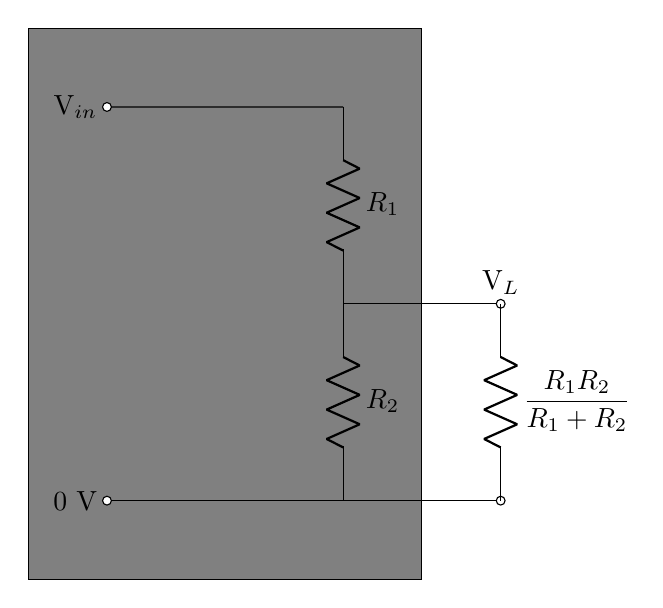
\begin{tikzpicture}
        % Gray backgorund box (can be commented out)
        \draw [fill=gray] (0,4.5) rectangle (5,11.5);
        % Voltage divider
        \draw (4,10.5) to[short,-o] (1,10.5); % Connect to 5 V DC
        \draw (1,10.5) node[anchor=east] {V$_{in}$};
        \draw  (4,10.5) to[R=$R_1$] (4,8);
        \draw (6,8) node[anchor=south] {V$_{L}$};
        \draw (4,8) to[short,-o] (6,8);
        \draw (4,8) to[R=$R_2$] (4,5.5);
        \draw (4,5.5) to[short,-o] (1,5.5); 
        \draw (1,5.5) node[anchor=east] {0 V};
        \draw (4,5.5) to[short,-o] (6,5.5);
        % Load resistor 
        \draw (6,8) to[R=$\dfrac{R_1 R_2}{R_1+R_2}$] (6,5.5);
    \end{tikzpicture}
    \end{figure}
\end{frame}
%%%%%%%%%%%%%%%%%%%%
\begin{frame}{\secname : \subsecname}
    Next, turning $R_{Load}$ and $R_2$ into an equivalent resistor
    \begin{figure}
    \begin{tikzpicture}
        % Voltage divider
        \draw (4,10.5) to[short,-o] (1,10.5); % Connect to 5 V DC
        \draw (1,10.5) node[anchor=east] {V$_{in}$};
        \draw  (4,10.5) to[R=$R_1$] (4,8);
        \draw (6,8) node[anchor=south] {V$_{L}$};
        \draw (4,8) to[short,-o] (6,8);
        \draw (4,8) to[R=$\textcolor{green}{R_2}$,color=green] (4,5.5);
        \draw (4,5.5) to[short,-o] (1,5.5); 
        \draw (1,5.5) node[anchor=east] {0 V};
        \draw (4,5.5) to[short,-o] (6,5.5);
        % Load resistor 
        \draw (6,8) to[R=$\textcolor{green}{\dfrac{R_1 R_2}{R_1+R_2}}$,color=green] (6,5.5);
    \end{tikzpicture}
    \end{figure}
\end{frame}
%%%%%%%%%%%%%%%%%%%%
\begin{frame}{\secname : \subsecname}
    \begin{equation}
        \dfrac{1}{R_{eq}}=\dfrac{1}{R_{2}}+\dfrac{1}{R_{th}}=\dfrac{1}{R_{2}}+\left( \dfrac{1}{R_{1}}+\dfrac{1}{R_{2}} \right) = \dfrac{2}{R_{2}}+\dfrac{1}{R_{1}}
    \end{equation}
    \begin{figure}
    \begin{tikzpicture}
        % Voltage divider
        \draw (4,10.5) to[short,-o] (1,10.5); % Connect to 5 V DC
        \draw (1,10.5) node[anchor=east] {V$_{in}$};
        \draw  (4,10.5) to[R=$R_1$] (4,8);
        \draw (6,8) node[anchor=south] {V$_{L}$};
        \draw (4,8) to[short,-o] (6,8);
        \draw (4,8) to[R=$\color{green}{R_{eq}}$,color=green] (4,5.5);
        \draw (4,5.5) to[short,-o] (1,5.5); 
        \draw (1,5.5) node[anchor=east] {0 V};
        \draw (4,5.5) to[short,-o] (6,5.5);
    \end{tikzpicture}
    \end{figure}
\end{frame}
%%%%%%%%%%%%%%%%%%%%
\begin{frame}{\secname : \subsecname}
    Then applying the voltage divider equation
    \begin{equation}
        V_{L}=\left( \dfrac{R_{eq}}{R_{eq}+R_{1}} \right) V_{in}
    \end{equation}
    \begin{figure}
    \begin{tikzpicture}
        % Voltage divider
        \draw (4,10.5) to[short,-o] (1,10.5); % Connect to 5 V DC
        \draw (1,10.5) node[anchor=east] {V$_{in}$};
        \draw  (4,10.5) to[R=$R_1$] (4,8);
        \draw (6,8) node[anchor=south] {V$_{L}$};
        \draw (4,8) to[short,-o] (6,8);
        \draw (4,8) to[R=$R_{eq}$] (4,5.5);
        \draw (4,5.5) to[short,-o] (1,5.5); 
        \draw (1,5.5) node[anchor=east] {0 V};
        \draw (4,5.5) to[short,-o] (6,5.5);
    \end{tikzpicture}
    \end{figure}
\end{frame}
%%%%%%%%%%%%%%%%%%%%
\begin{frame}{\secname : \subsecname}
    Simplifying using algebra:
    \begin{align}
        V_{L} &= \left( \dfrac{R_{eq}}{R_{eq}+R_1} \right) V_{in} \\
                &= \left( \dfrac{R_{eq} R_1}{R_{eq}+R_1} \right) \dfrac{V_{in}}{R_1} \\
                &= \left( \dfrac{1}{R_1} + \dfrac{1}{R_{eq}} \right)^{-1} \dfrac{V_{in}}{R_1} \\ 
                &= \left( \dfrac{1}{R_1} + \dfrac{2}{R_{2}}+\dfrac{1}{R_{1}} \right)^{-1} \dfrac{V_{in}}{R_1} \\
                &= \left( \dfrac{2}{R_1} + \dfrac{2}{R_{2}} \right)^{-1} \dfrac{V_{in}}{R_1} \\
                &= \left( \dfrac{R_1 R_2}{R_1+R_2} \right) \dfrac{V_{in}}{2 R_1} \\
            V_L &= \left( \dfrac{R_2}{R_1+R_2} \right) \dfrac{V_{in}}{2} = \dfrac{V_{out}}{2}
    \end{align}
\end{frame}
%%%%%%%%%%%%%%%%%%%%
\subsection{The Loading Problem}
%%%%%%%%%%%%%%%%%%%%
\begin{frame}{\secname : \subsecname}
    Any circuit can be split into a Source and a Load.
    \begin{figure}
    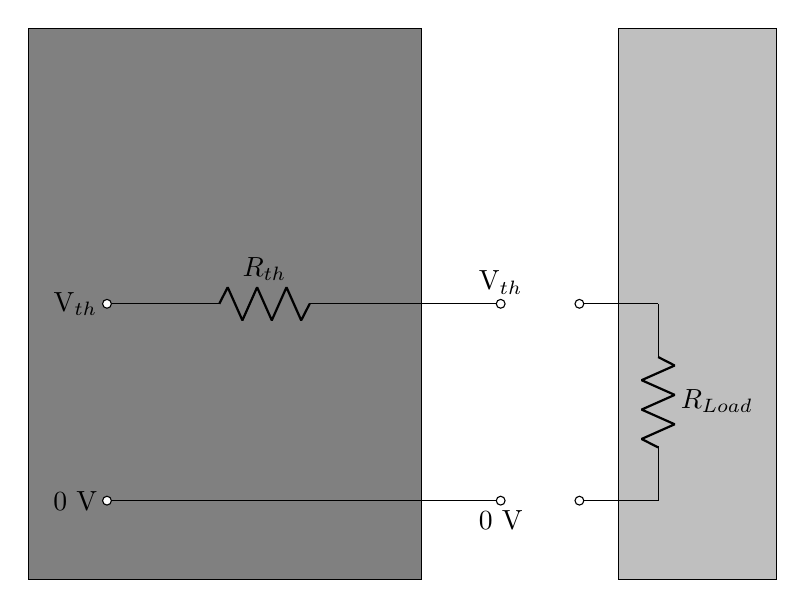
\begin{tikzpicture}
        % Source
        % Gray backgorund box (can be commented out)
        \draw [fill=gray] (0,4.5) rectangle (5,11.5);
        \draw (2,8) to [short,-o] (1,8);
        \draw (2,8) to[R=$R_{th}$] (4,8); % Connect to 5 V DC
        \draw (1,8) node[anchor=east] {V$_{th}$};
        \draw (4,8) to[short,-o] (6,8);
        \draw (4,5.5) to[short,-o] (1,5.5); 
        \draw (1,5.5) node[anchor=east] {0 V};
        \draw (4,5.5) to[short,-o] (6,5.5);
        \draw (6,8) node[anchor=south] {V$_{th}$};
        \draw (6,5.5) node[anchor=north] {0 V};
        % Load 
        \draw [fill=lightgray] (7.5,4.5) rectangle (9.5,11.5);
        \draw (8,5.5) to[short,-o](7,5.5);
        \draw (8,8) to[short,-o](7,8);
        \draw (8,8) to[R=$R_{Load}$] (8,5.5);
    \end{tikzpicture}
    \end{figure}
\end{frame}
%%%%%%%%%%%%%%%%%%%%
\begin{frame}{\secname : \subsecname}
    \textcolor{red}{But connecting them changes the voltage.}
    \begin{figure}
    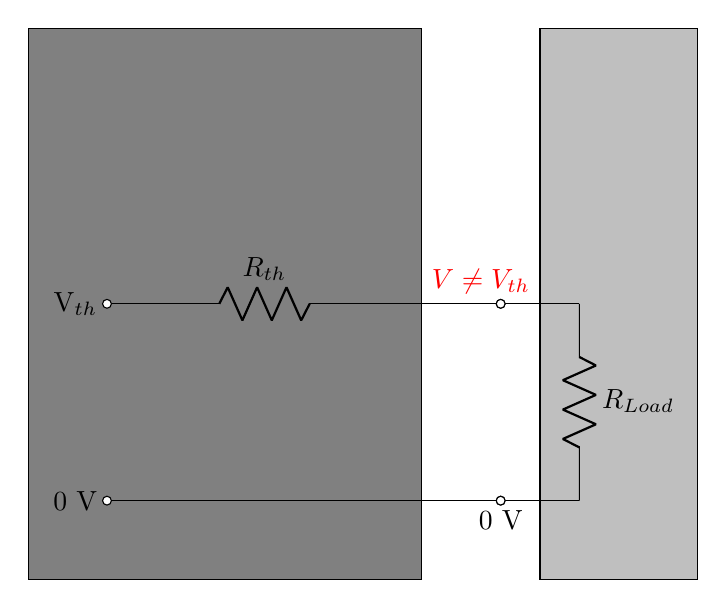
\begin{tikzpicture}
        % Source
        % Gray backgorund box (can be commented out)
        \draw [fill=gray] (0,4.5) rectangle (5,11.5);
        \draw (2,8) to [short,-o] (1,8);
        \draw (2,8) to[R=$R_{th}$] (4,8); % Connect to 5 V DC
        \draw (1,8) node[anchor=east] {V$_{th}$};
        \draw (4,8) to[short,-o] (6,8);
        \draw (4,5.5) to[short,-o] (1,5.5); 
        \draw (1,5.5) node[anchor=east] {0 V};
        \draw (4,5.5) to[short,-o] (6,5.5);
        \draw (5.75,8) node[anchor=south] {$\textcolor{red}{V \ne V_{th}}$};
        \draw (6,5.5) node[anchor=north] {0 V};
        % Load 
        \draw [fill=lightgray] (6.5,4.5) rectangle (8.5,11.5);
        \draw (7,5.5) to[short,-o](6,5.5);
        \draw (7,8) to[short,-o](6,8);
        \draw (7,8) to[R=$R_{Load}$] (7,5.5);
    \end{tikzpicture}
    \end{figure}
\end{frame}
%%%%%%%%%%%%%%%%%%%%
\begin{frame}{\secname : \subsecname}
    We need a ``matchmaker": a component that \\
    looks like a high resistance when viewed from the Source, but \\
    looks like a low resistance when viewed from the Load.
    \begin{figure}
    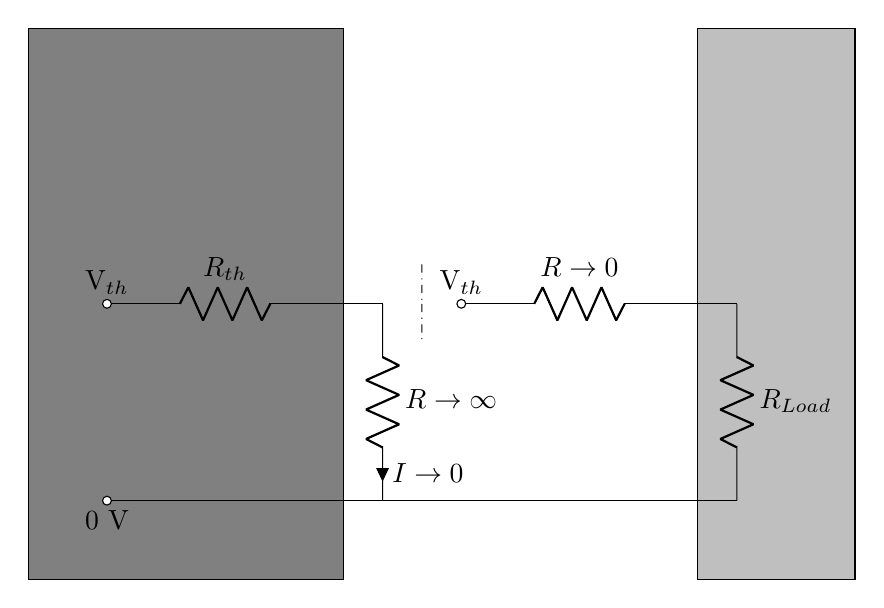
\begin{tikzpicture}
        % Matchmaker
        %\draw [fill=yellow] (4,4.5) rectangle (8.5,11.5);
        \draw (4.5,8) to[R=$R \rightarrow \infty$,i^=$I \rightarrow 0$] (4.5,5.5); 
        \draw (6,8) to [short,-o] (5.5,8);
        \draw (6,8) to[R=$R \rightarrow 0$] (8,8); 
        \draw (5.5,8) node[anchor=south] {V$_{th}$};
        \draw (4.5,5.5) to[short,-] (8,5.5);
        \draw [dash dot] (5,8.5) to [short,-] (5,7.5);
        % Source
        \draw [fill=gray] (0,4.5) rectangle (4,11.5);
        \draw (1.5,8) to [short,-o] (1,8);
        \draw (1.5,8) to[R=$R_{th}$] (3.5,8); 
        \draw (1,8) node[anchor=south] {V$_{th}$};
        \draw (3.5,8) to[short,-] (4.5,8);
        \draw (3.5,5.5) to[short,-o] (1,5.5); 
        \draw (1,5.5) node[anchor=north] {0 V};
        \draw (3.5,5.5) to[short,-] (4.5,5.5);
        % Load 
        \draw [fill=lightgray] (8.5,4.5) rectangle (10.5,11.5);
        \draw (9,5.5) to[short,-](8,5.5);
        \draw (9,8) to[short,-](8,8);
        \draw (9,8) to[R=$R_{Load}$] (9,5.5);
    \end{tikzpicture}
    \end{figure}
\end{frame}
%%%%%%%%%%%%%%%%%%%%
\section{The Op Amp}
%%%%%%%%%%%%%%%%%%%%
\subsection{Basic Properties}
%%%%%%%%%%%%%%%%%%%%
\begin{frame}{\secname : \subsecname}
    The input leads draw no current \\
    The output has zero source resistance \\
    The output output attempts to make the input voltages the same
    \begin{figure}
    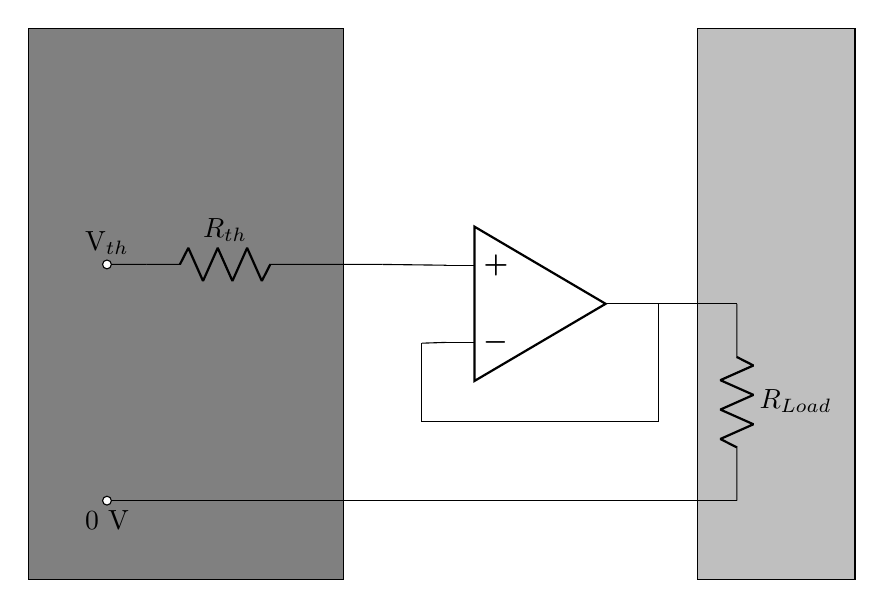
\begin{tikzpicture}
        % Matchmaker
        \draw (6.5,8) node[op amp,yscale=-1](opamp1) {};
        \draw (opamp1.+) to[short,-] (4.5,8.5);
        \draw (opamp1.-) to[short,-] (5,7.5);
        \draw (opamp1.out) to[short,-] (8,8);
        \draw (5,7.5) -- (5,6.5) -- (8,6.5) -- (8,8);
        % Source
        \draw [fill=gray] (0,4.5) rectangle (4,11.5);
        \draw (1.5,8.5) to [short,-o] (1,8.5);
        \draw (1.5,8.5) to[R=$R_{th}$] (3.5,8.5); 
        \draw (1,8.5) node[anchor=south] {V$_{th}$};
        \draw (3.5,8.5) to[short,-] (4.5,8.5);
        \draw (3.5,5.5) to[short,-o] (1,5.5); 
        \draw (1,5.5) node[anchor=north] {0 V};
        \draw (3.5,5.5) to[short,-] (4.5,5.5);
        % Load 
        \draw [fill=lightgray] (8.5,4.5) rectangle (10.5,11.5);
        \draw (9,5.5) to[short,-](4.5,5.5);
        \draw (9,8) to[short,-](8,8);
        \draw (9,8) to[R=$R_{Load}$] (9,5.5);
    \end{tikzpicture}
    \end{figure}
\end{frame}
%%%%%%%%%%%%%%%%%%%%
\subsection{Follower/Buffer}
%%%%%%%%%%%%%%%%%%%%
\begin{frame}{\secname : \subsecname}
    \begin{equation*}
        V_{out} = V_{in}
    \end{equation*}
    \begin{figure}
    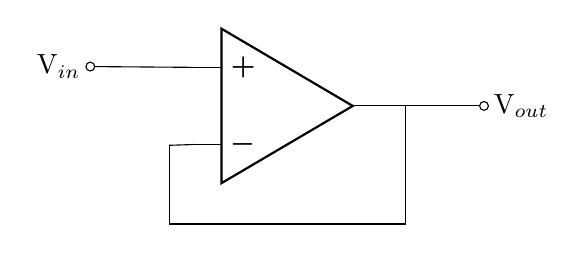
\begin{tikzpicture}
        % Matchmaker
        \draw (6.5,8) node[op amp,yscale=-1](opamp1) {};
        \draw (opamp1.+) to[short,-o] (4,8.5);
        \draw (opamp1.-) to[short,-] (5,7.5);
        \draw (opamp1.out) to[short,-o] (9,8);
        \draw (5,7.5) -- (5,6.5) -- (8,6.5) -- (8,8);
        \draw (4,8.5) node[anchor=east] {V$_{in}$};
        \draw (9,8) node[anchor=west] {V$_{out}$};
    \end{tikzpicture}
    \end{figure}
\end{frame}
%%%%%%%%%%%%%%%%%%%%
\subsection{Comparator}
%%%%%%%%%%%%%%%%%%%%
\begin{frame}{\secname : \subsecname}
\begin{equation*}
  V_{out} \rightarrow  \begin{cases}
    HIGH, & \text{if $V_{in}>V_{ref}$}.\\
    LOW, & \text{if $V_{in}<V_{ref}$}.
  \end{cases}
\end{equation*}
    \begin{figure}
    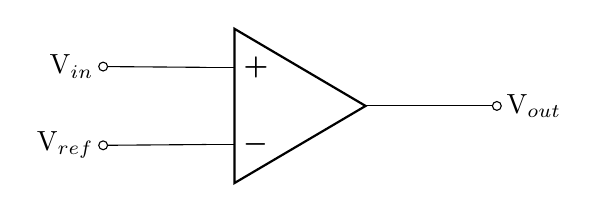
\begin{tikzpicture}
        % Matchmaker
        \draw (6.5,8) node[op amp,yscale=-1](opamp1) {};
        \draw (opamp1.+) to[short,-o] (4,8.5);
        \draw (opamp1.-) to[short,-o] (4,7.5);
        \draw (opamp1.out) to[short,-o] (9,8);
        \draw (4,8.5) node[anchor=east] {V$_{in}$};
        \draw (4,7.5) node[anchor=east] {V$_{ref}$};
        \draw (9,8) node[anchor=west] {V$_{out}$};
    \end{tikzpicture}
    \end{figure}
\end{frame}
%%%%%%%%%%%%%%%%%%%%
\subsection{Amplifier (non-inverting)}
%%%%%%%%%%%%%%%%%%%%
\begin{frame}{\secname : \subsecname}
\begin{equation*}
  V_{out} = \left( 1 + \dfrac{R_1}{R_2} \right) V_{in}
\end{equation*}
    \begin{figure}
    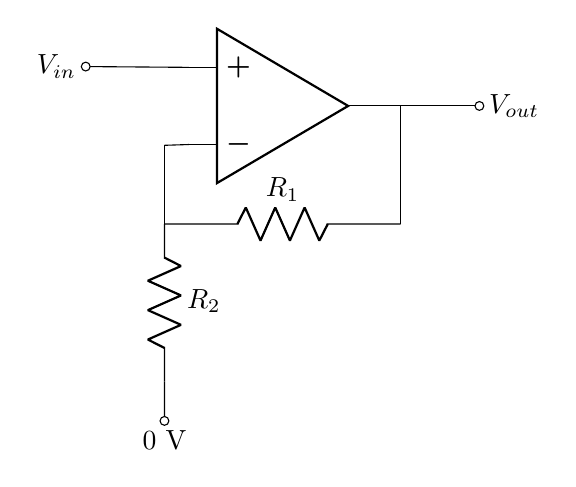
\begin{tikzpicture}
        \draw (6.5,8) node[op amp,yscale=-1](opamp1) {};
        \draw (opamp1.+) to[short,-o] (4,8.5);
        \draw (opamp1.-) to[short,-] (5,7.5);
        \draw (opamp1.out) to[short,-o] (9,8);
        \draw (5,7.5) -- (5,6.5);
        \draw (5,6.5) to[R=$R_1$] (8,6.5); 
        \draw (8,6.5) -- (8,8);
        \draw (5,6.5) to[R=$R_2$] (5,4.5);
        \draw (5,4.5) to[short,-o] (5,4);
        \draw (5,4) node[anchor=north] {0 V};
        \draw (4,8.5) node[anchor=east] {$V_{in}$};
        \draw (9,8) node[anchor=west] {$V_{out}$};
    \end{tikzpicture}
    \end{figure}
\end{frame}
%%%%%%%%%%%%%%%%%%%%
\end{document}